Two methods have been studied and implemented to regulate the pack of robots. The first approach is a method based on artificial potentials field. This method is robust and easy to debug. It was chosen to regulate the real robots on the testing field because it was easier to implement on the robots and provided good results. The second one is a method of feedback linearisation. This method was chosen for the simulation of the surveillance of the Bay of Biscay because it is a classic and efficient method.

\subsection{Artificial Potentials Field}
\vspace*{0.5 cm}
\textcolor{blue} {Thomas Boulier \& Sylvain Hunault}
\vspace*{0.5cm}

Let $p_{robot}$ be the position of our considered robot, let $p_{target}$ and $v_{target}$ be the position and speed of the target we want the robot to reach.
We can consider the robot and the target as two particles of opposite charge, and then compute the potentials field between them. In case of obstacles, we can consider them as particles of same charge than the robot's.
The potentials field method calculates the instantaneous speed vector $w(p_{robot},t)$ the robot needs to reach (or at least follow) the target. To compute that speed, we use the potential $V$ between the robot and the target :\\
\[ V(p_{robot}) = v^T_{target}. p_{robot} + \|p_{robot}-p_{target}\|^2 \]
And compute the gradient of that potential to find the order $w(p_{robot},t)$:
\[w(p_{robot},t) = -grad(V(p_{robot})) = -\frac{dV}{dP}(p)^T\]
So :
\[w(p_{robot},t) = v_{target}-2.(p_{robot}-p_{target})\]
For $w$, we compute the order speed and course:
\[\bar{v} = \|w\| \]
\[\bar{\theta} = tan(\frac{w_y}{w_x})\]

As illustrated in the picture below, a proportional regulation computes the command $u_v$ and $u_{\theta}$ which will be used to control the robot.

\[ u_v = Kp_v \cdot (\bar{v}-v_{robot}) \]
\[ u_{\theta} = Kp_{\theta} \cdot (\bar{\theta}-\theta_{robot}) \]

Where $\theta_{robot}$ is the course of the robot calculated by finite difference because the GPS of the robot do not provide the course.

\begin{figure}[H]
\centering
   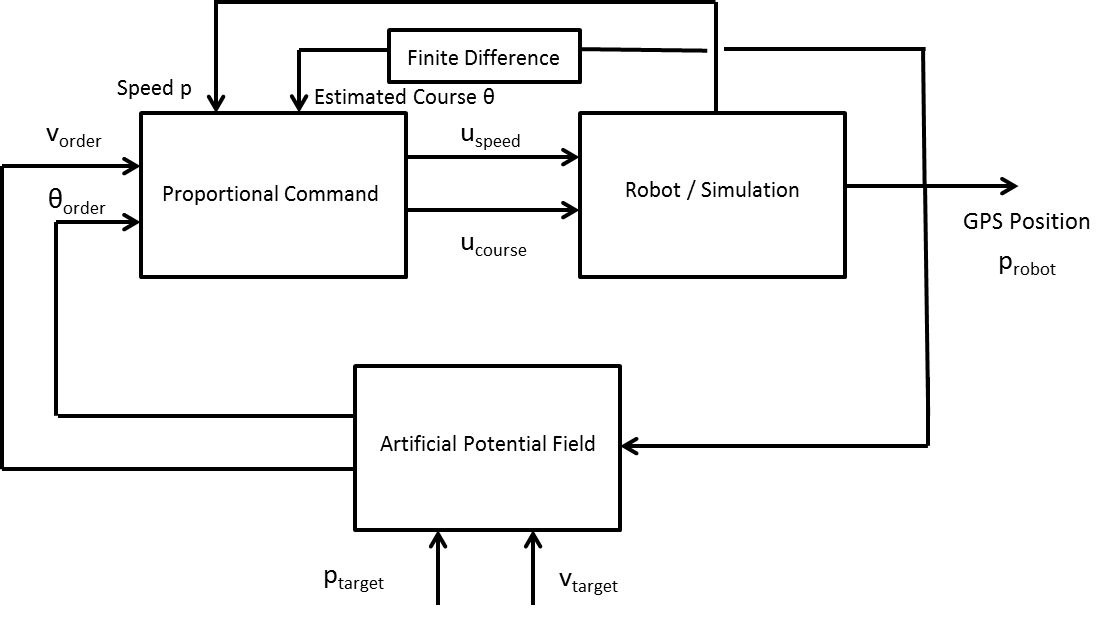
\includegraphics[scale=0.5]{schema_regulation_potentiels.png}
   \caption{\label{schema_regulation_potentiels} Architecture of the potentials field method}
\end{figure}

$u_v$ and $u_{\theta}$ are saturated to avoid an overloading of the actuators.\\

This command is then used as the entry of a simple simulator used to test the regulation.
The command is used as the acceleration of the robot, and its position at each time is computed through an Euler method. The objective point is on an parametric ellipse moving with time.\\

The method is easily extended to multiple robots : each one is controlled separately. For each iteration of the loop, the regulation process is applied on each robot. The command is calculated for each one, then the simulation uses it to compute the new position of each one.

$u_v$ and $u_{\theta}$ are saturated to avoid a surcharge of the actuators. 

\subsection{Feedback Linearisation}
\vspace*{0.5 cm}
	\textcolor{blue} {Alice Danckaers}
\vspace*{0.5cm}

Feedback linearisation is a classical approach used in controlling nonlinear systems. We transform the nonlinear system \ref{system1} into an equivalent linear system \ref{system2}, which is of the form $\ddot{y}=A(x)*u$.

\begin{equation}
\dot{x} = f(x,u) \rightarrow \left\{ 
\begin{array}{l l}
  \dot{x_1} = x_4 * \cos(x_3)\\
  \dot{x_2} = x_4 * \sin(x_3)\\
  \dot{x_3} = u_1\\
  \dot{x_4} = u_2\\
\end{array} \right.
\label{system1}
\end{equation}

\begin{equation}
\begin{pmatrix}
	\ddot{y_1}\\
	\ddot{y_2} 
\end{pmatrix}
=
\begin{pmatrix}
	-x_4*\sin(x_3) & \cos(x_3)\\
	 x_4*\cos(x_3) & \sin(x_3)
\end{pmatrix}
\begin{pmatrix}
	u_1\\
	u_2
\end{pmatrix}   
\hspace*{1cm} \textnormal{ with } y = \begin{pmatrix}
	x_1\\
	x_2
\end{pmatrix}
\label{system2}
\end{equation}

If $w$ is the instruction of the robot has to follow, then we have the expression of the command $u$ as shown in equation \ref{equationU}. We can then use it to regulate the robot in an Euler method.
\begin{equation}
 u =
\begin{pmatrix}
	-x_4*\sin(x_3) & \cos(x_3)\\
	 x_4*\cos(x_3) & \sin(x_3)
\end{pmatrix}^{-1}
\begin{pmatrix}
	(y_1-w_1) + (\dot{y_1} - \dot{w_1}) -  \ddot{w_1}\\
	(y_2-w_2) + (\dot{y_2} - \dot{w_2}) -  \ddot{w_2}
\end{pmatrix}
\label{equationU}
\end{equation}
